\documentclass{beamer}
\usetheme{Berlin}

\title{Systems with a Small Number of
Variables}
\subtitle{Course: Complex Systems Modeling}
\author{Robert Flassig}
\institute{Brandenburg University of Applied Sciences}
\date{\today}

\begin{document}
\begin{frame}
\titlepage
\end{frame}

\begin{frame}
\frametitle{Outline}
\tableofcontents
\end{frame}

\section{Continuous-Time Models: Analysis}
\begin{frame}
\frametitle{Equilibrium Points}

\begin{block}{Definition}
Equilibrium points of a continuous-time model \(\frac{dx}{dt} = F(x)\) are found by solving:
\[
0 = F(x_{\text{eq}})
\]
\end{block}

\begin{itemize}
    \item At equilibrium, the system's state does not change over time.
    \item Example: Logistic growth model:
    \[
    \frac{dx}{dt} = r x \left(1 - \frac{x}{K}\right)
    \]
    Equilibrium points:
    \[
    x_{\text{eq}} = 0, \quad x_{\text{eq}} = K
    \]
\end{itemize}

\end{frame}

\begin{frame}
\frametitle{Phase Space Analysis}

\begin{block}{Phase Space}
The phase space represents the state of the system as a trajectory in a coordinate space.
\end{block}

\begin{itemize}
    \item Continuous-time models have smooth trajectories in phase space.
    \item Key features:
    \begin{itemize}
        \item Equilibrium points: Points where \(\frac{dx}{dt} = 0\).
        \item Trajectory directions: Show how the state evolves over time.
    \end{itemize}
    \item Example: A predator-prey model:
    \[
    \frac{dx}{dt} = x - xy, \quad \frac{dy}{dt} = -y + xy
    \]
    The trajectories rotate around equilibrium points.
\end{itemize}

\end{frame}

\begin{frame}
\frametitle{Example: Phase Space Analysis}

\begin{figure}[htbp]
    \centering
    \begin{minipage}{0.48\textwidth}
        \centering
        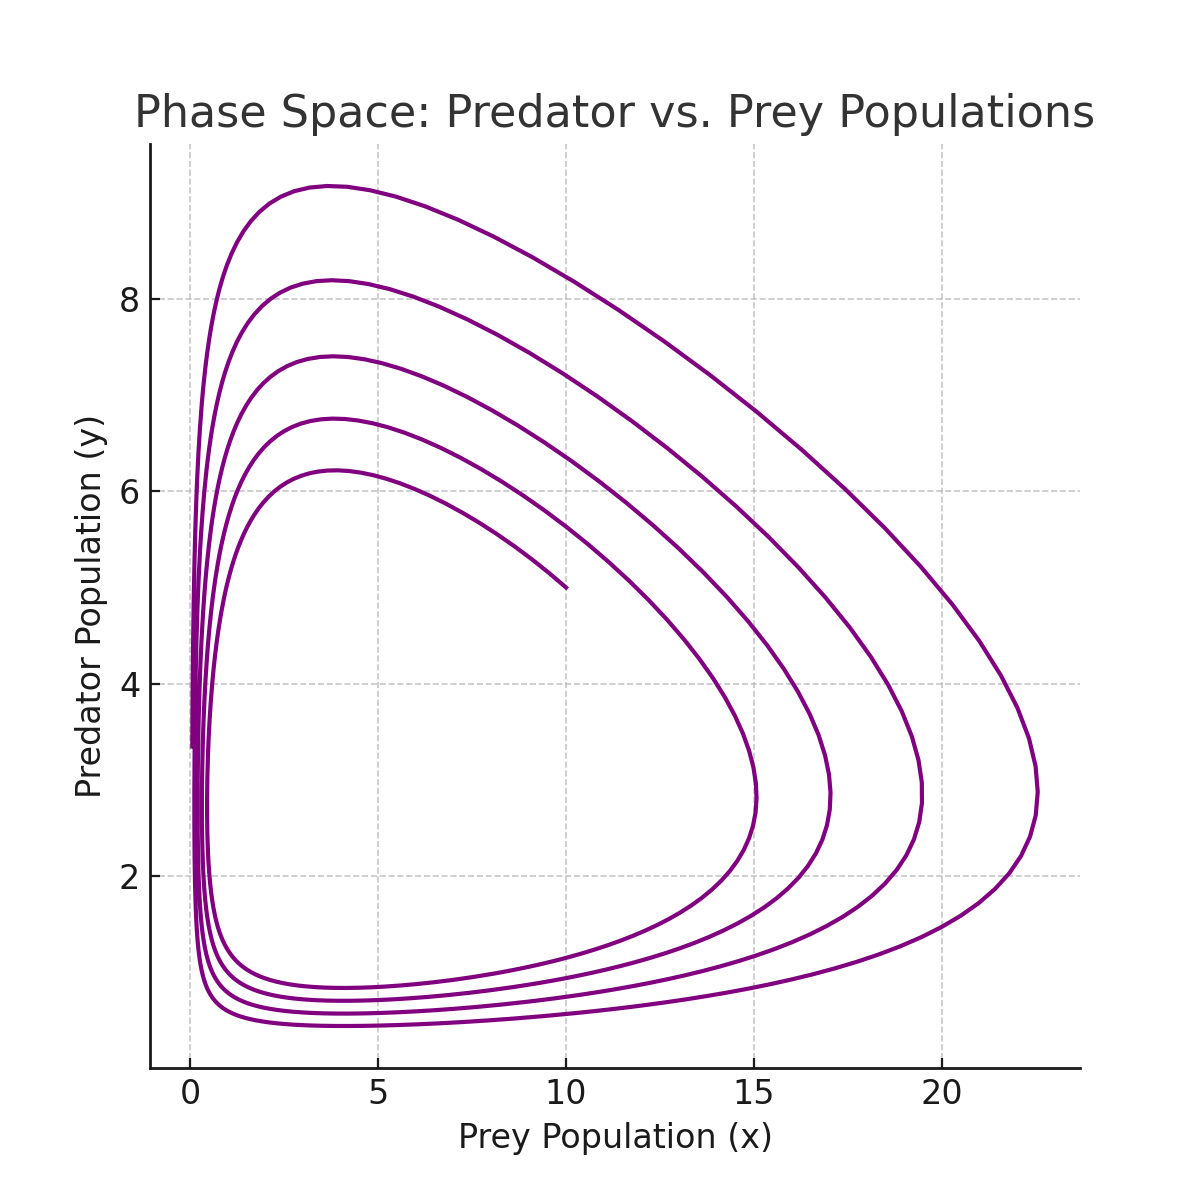
\includegraphics[width=\textwidth]{lotka_volterra_phase_space.png}
        \caption{Phase space representation of the Lotka–Volterra system.}
        \label{fig:lotka_volterra_phase_space}
    \end{minipage}
    \hfill
    \begin{minipage}{0.48\textwidth}
        \centering
        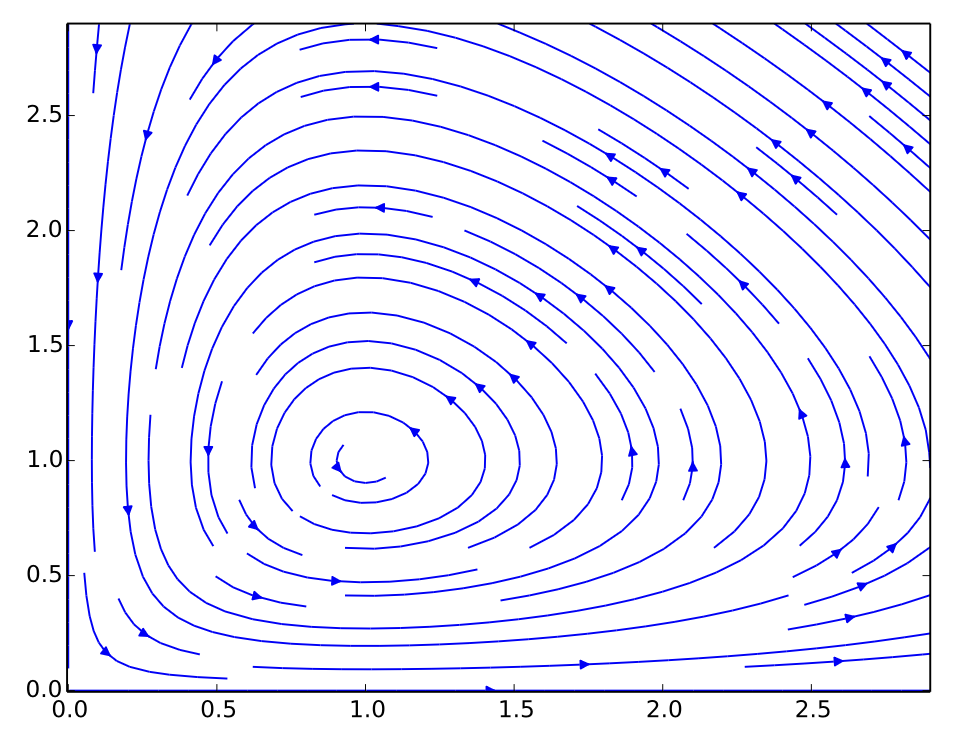
\includegraphics[width=\textwidth]{lotka_volterra_phase_space_02.png}
        \caption{Alternative phase space trajectory visualization. Credit: H. Sayama, \emph{Introduction to the Modeling and Analysis of Complex Systems}, 2015 (CC BY-NC-SA)}
        \label{fig:lotka_volterra_phase_space_02}
    \end{minipage}
\end{figure}

\end{frame}



\begin{frame}
\frametitle{Nullclines}

\begin{block}{Definition}
A nullcline is a set of points where one of the time derivatives becomes zero.
\end{block}

\begin{itemize}
    \item For \(\frac{dx}{dt} = 0\): Horizontal movement stops, trajectories flow vertically.
    \item For \(\frac{dy}{dt} = 0\): Vertical movement stops, trajectories flow horizontally.
    \item Intersection points of nullclines are equilibrium points.
\end{itemize}

\end{frame}


\begin{frame}
\frametitle{Nullclines}

\begin{block}{Example: Lotka-Volterra Model}
\[
\frac{dx}{dt} = ax - bxy, \quad \frac{dy}{dt} = -cy + dxy
\]
\begin{itemize}
    \item Nullclines:
    \[
    x = 0 \, \text{or} \, y = \frac{a}{b}, \quad y = 0 \, \text{or} \, x = \frac{c}{d}
    \]
\end{itemize}
\end{block}

\end{frame}


\begin{frame}
\frametitle{Nullclines}

\begin{figure}[htbp]
    \centering
    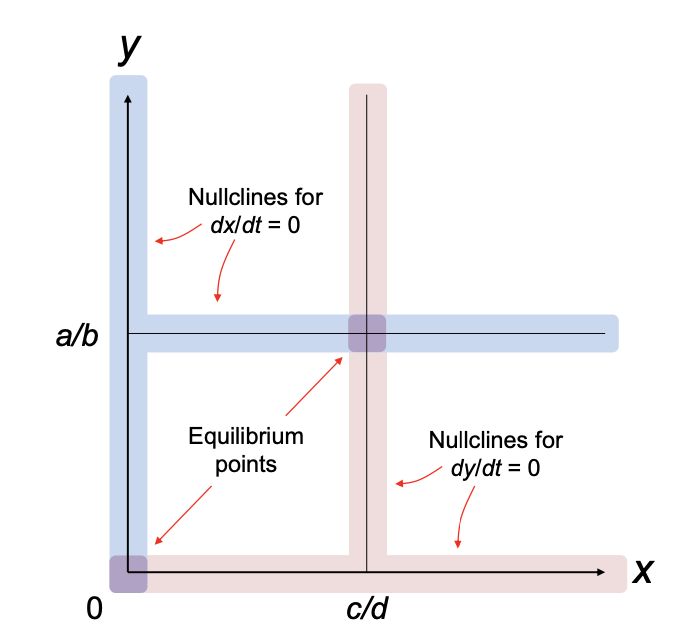
\includegraphics[width=0.5\textwidth]{nullclines_a.png}
    \caption{Nullclines according to the above equations (conditions). Credit: H. Sayama, 2015 (CC BY-NC-SA)}
    \label{fig:nullclines_a}
\end{figure}

\end{frame}


\begin{frame}
\frametitle{Nullclines}

\begin{figure}[htbp]
    \centering
    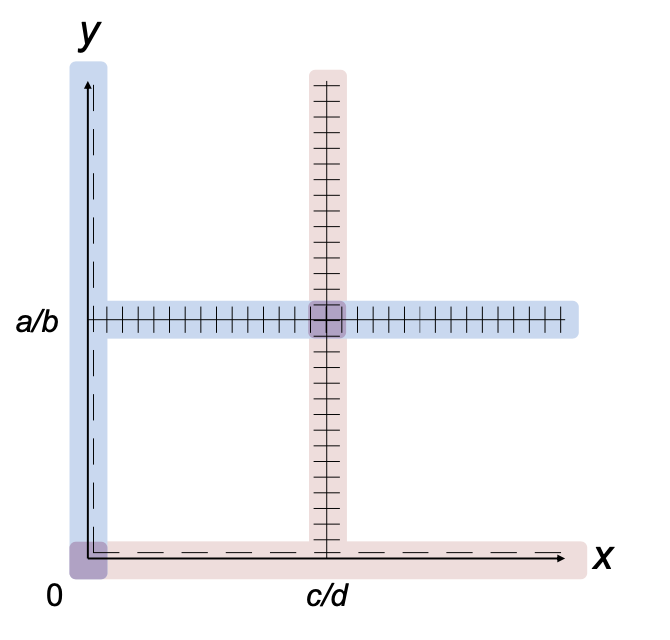
\includegraphics[width=0.5\textwidth]{nullclines_b.png}
    \caption{Nullclines with added directions. Credit: H. Sayama, 2015 (CC BY-NC-SA)}
    \label{fig:nullclines_b}
\end{figure}


\end{frame}



\begin{frame}
\frametitle{Phase Space Regions and Trajectory Directions}

\begin{block}{Phase Space Division}
The phase space is divided into four regions, with trajectories in each region flowing in one of four directions:
\begin{itemize}
    \item Northeast: \(\frac{dx}{dt} > 0, \frac{dy}{dt} > 0\)
    \item Northwest: \(\frac{dx}{dt} < 0, \frac{dy}{dt} > 0\)
    \item Southeast: \(\frac{dx}{dt} > 0, \frac{dy}{dt} < 0\)
    \item Southwest: \(\frac{dx}{dt} < 0, \frac{dy}{dt} < 0\)
\end{itemize}
\end{block}

\begin{itemize}
    \item Trajectories in a region never switch between these directional categories.
    \item Any switching would appear as part of the nullclines.
\end{itemize}



\end{frame}

\begin{frame}
\frametitle{Nullclines}

\begin{figure}[htbp]
    \centering
    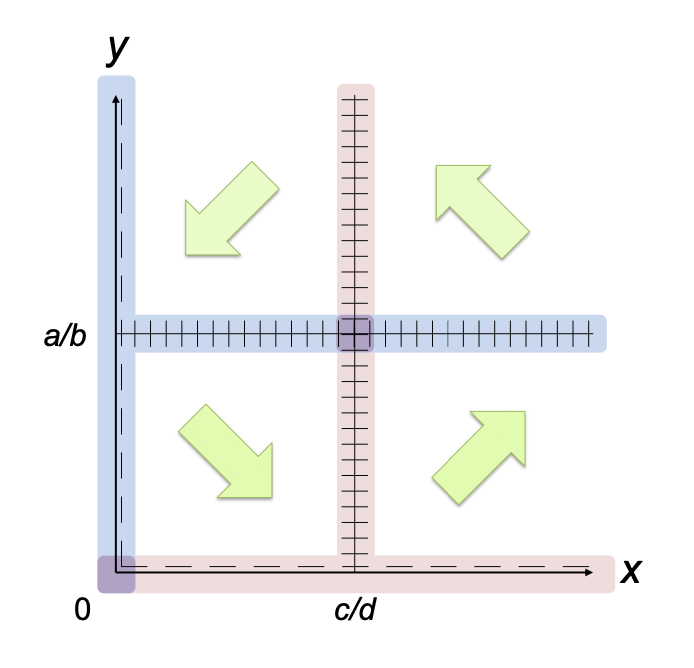
\includegraphics[width=0.5\textwidth]{nullclines_c.png}
    \caption{Directions inside the nullclines. Credit: H. Sayama, 2015 (CC BY-NC-SA)}
    \label{fig:nullclines_c}
\end{figure}


\end{frame}



\begin{frame}
\frametitle{Testing Directions in Regions}
\small
\begin{itemize}
    \item Sample a point from each region and test its trajectory direction using the model equations.
    \item Example: Upper-right region (\((x, y) = (\frac{2c}{d}, \frac{2a}{b})\)).
\end{itemize}

\begin{block}{Trajectory Calculation}
\begin{align*}
\frac{dx}{dt} \big|_{(x, y) = (\frac{2c}{d}, \frac{2a}{b})} &= a \frac{2c}{d} - b \frac{2c}{d} \frac{2a}{b} = -\frac{2ac}{d} < 0 \\
\frac{dy}{dt} \big|_{(x, y) = (\frac{2c}{d}, \frac{2a}{b})} &= -c \frac{2a}{b} + d \frac{2c}{d} \frac{2a}{b} = \frac{2ac}{b} > 0
\end{align*}
\end{block}

\begin{itemize}
    \item Direction: Northwest (\(\frac{dx}{dt} < 0, \frac{dy}{dt} > 0\)).
    \item Repeat for other regions to outline the full phase space behavior.
\end{itemize}

\begin{block}{Cyclic Behavior}
The resulting phase space shows cyclic behavior caused by predator-prey interactions.
\end{block}

\end{frame}

\begin{frame}
\frametitle{Predator-Prey Model Phase Space}

\begin{block}{Equations}
\[
\frac{dx}{dt} = x - xy, \quad \frac{dy}{dt} = -y + xy
\]
\end{block}

\begin{itemize}
    \item Nullclines:
    \[
    \frac{dx}{dt} = 0 \implies y = 1, \quad \frac{dy}{dt} = 0 \implies x = 1
    \]
    \item Equilibrium point: \((x, y) = (1, 1)\)
    \item Trajectories rotate around the equilibrium point in a cyclic manner.
\end{itemize}

\end{frame}

\begin{frame}
\frametitle{Summary}

\begin{itemize}
    \item Equilibrium Points:
    \begin{itemize}
        \item Found by solving \(\frac{dx}{dt} = 0\).
        \item Indicate steady-state solutions.
    \end{itemize}
    \item Phase Space:
    \begin{itemize}
        \item Visualizes system behavior over time.
        \item Shows trajectories and flow of the state.
    \end{itemize}
    \item Nullclines:
    \begin{itemize}
        \item Identify where movement stops in one direction.
        \item Separate the phase space into regions.
    \end{itemize}
\end{itemize}

\begin{block}{Practical Use}
Combine these tools to understand and predict the dynamics of continuous-time systems.
\end{block}

\end{frame}

\section{Exercise}
\begin{frame}
\scriptsize
\frametitle{Equilibrium Points of \(\frac{dx}{dt} = x^2 - rx + 1\)}

\begin{block}{Given Model}
\[
\frac{dx}{dt} = x^2 - rx + 1
\]
\end{block}

\begin{itemize}
    \item Step 1: Set \(\frac{dx}{dt} = 0\):
    \[
    {x^*}^2 - rx^* + 1 = 0
    \]
    \item Step 2: Solve the quadratic equation:
    \[
    x^*_{\pm} = \frac{r \pm \sqrt{r^2 - 4}}{2}
    \]
    \item Real solutions exist only if \(r^2 \geq 4\).
\end{itemize}

\begin{block}{Equilibrium Points}
\[
x^*_+ = \frac{r + \sqrt{r^2 - 4}}{2}, \quad x^*_{-} = \frac{r - \sqrt{r^2 - 4}}{2}
\]
\end{block}

\end{frame}

\begin{frame}
\frametitle{Equilibrium Points of a Simple Pendulum}
\small
\begin{block}{Model}
\[
\frac{d^2\theta}{dt^2} = -\frac{g}{L}\sin\theta
\]
\end{block}

\begin{columns}[T,totalwidth=\textwidth]
\begin{column}{0.5\textwidth}
\textbf{Step 1: First-Order System}
\[
\omega = \frac{d\theta}{dt}, \qquad 
\frac{d\omega}{dt} = -\frac{g}{L}\sin\theta
\]
\vspace{1em}
\textbf{Step 2: Equilibrium Conditions}
\[
\frac{d\theta}{dt} = 0, \qquad 
\frac{d\omega}{dt} = 0
\]
\end{column}
\begin{column}{0.5\textwidth}
\textbf{Step 3: Solve}
\[
\omega^* = 0, \quad \sin\theta^* = 0 
\implies \theta^* = n\pi, \; n \in \mathbb{Z}
\]
\begin{block}{Equilibria}
\[
(\theta^*, \omega^*) = (n\pi, 0), \quad n \in \mathbb{Z}
\]
\end{block}
\end{column}
\end{columns}
\end{frame}


\begin{frame}
\frametitle{Equilibrium Points of the SIR Model (1/2)}
\small
\begin{block}{Model}
\[
\begin{aligned}
\frac{dS}{dt} &= -aSI, \qquad
\frac{dI}{dt} = aSI - bI, \qquad
\frac{dR}{dt} = bI
\end{aligned}
\]
\end{block}

\begin{columns}[T,totalwidth=\textwidth]
\begin{column}{0.55\textwidth}
\textbf{Step 1: Equilibrium Conditions}
\[
\frac{dS}{dt} = 0, \quad 
\frac{dI}{dt} = 0, \quad 
\frac{dR}{dt} = 0
\]

\textbf{Step 2: From } $\frac{dS}{dt}=0$
\[
-aSI = 0 \implies S=0 \text{ or } I=0
\]
\end{column}

\begin{column}{0.45\textwidth}
\textbf{From } $\frac{dI}{dt}=0$
\[
aSI - bI = 0 \implies I(aS-b)=0
\]
\[
\Rightarrow I=0 \text{ or } S = \frac{b}{a}
\]

\textbf{From } $\frac{dR}{dt}=0$
\[
bI = 0 \implies I=0
\]
(no new constraint)
\end{column}
\end{columns}
\end{frame}


\begin{frame}
\frametitle{Equilibrium Points of the SIR Model (2/2)}
\small
\begin{block}{Equilibria}
\[
\begin{aligned}
&(1)\quad (S^*, I^*, R^*) = (S_0, 0, R_0) 
&&\text{(Disease-free equilibrium)} \\[4pt]
&(2)\quad (S^*, I^*, R^*) = \left(\frac{b}{a}, 0, R_0 + S_0 - \frac{b}{a}\right)
&&\text{(Endemic equilibrium, if } S_0 > \tfrac{b}{a})
\end{aligned}
\]
\end{block}

\begin{itemize}
\item Both equilibria satisfy $I^* = 0$.
\item The second case exists only if the infection can spread, i.e. $R_0 = \frac{aS_0}{b} > 1$.
\end{itemize}
\end{frame}


\begin{frame}
\frametitle{Exercise: Nullclines of the SIR Model}

\tiny
\begin{block}{}
Draw an outline of the phase space of the following SIR model
(variable \( R \) omitted) by studying the nullclines and estimating the directions
of trajectories within each region separated by those nullclines.
\end{block}

\[
\begin{aligned}
\frac{dS}{dt} &= -aSI \\
\frac{dI}{dt} &= aSI - bI
\end{aligned}
\]

\[
S \ge 0, \quad I \ge 0, \quad a>0, \quad b>0
\]

\begin{block}{Nullclines}
\[
\begin{aligned}
\frac{dS}{dt} = 0 &\Rightarrow S=0 \text{ or } I=0, \\
\frac{dI}{dt} = 0 &\Rightarrow I=0 \text{ or } S = \frac{b}{a}.
\end{aligned}
\]
\end{block}

\end{frame}


\begin{frame}
\frametitle{Exercise: Nullclines of a Nonlinear Oscillator}

\tiny
\begin{block}{}
Draw an outline of the phase space of the following nonlinear system
by studying nullclines and estimating the directions of trajectories within
each region separated by those nullclines.
\end{block}

\[
\frac{d^2x}{dt^2} - x\frac{dx}{dt} + x^2 = 0
\]

Let \( y = \frac{dx}{dt} \), then
\[
\frac{dx}{dt} = y, \qquad \frac{dy}{dt} = xy - x^2.
\]

\begin{block}{Nullclines}
\[
\begin{aligned}
\frac{dx}{dt} = 0 &\Rightarrow y = 0, \\
\frac{dy}{dt} = 0 &\Rightarrow x(y - x) = 0 \Rightarrow x=0 \text{ or } y=x.
\end{aligned}
\]
\end{block}

\end{frame}


\section{Asymptotic Analysis}

\begin{frame}

\emph{Asymptotic Stability Analysis} -- continued in the next lectures.
\end{frame}

\end{document}